%%%%%%%%%%%%%%%%%%%%%%%%%%%%%%%%%%%%%%%%%%%%%%%%%%%%%%%%%%%%%%%%%%%%%%%%%%%%%%%%%%%%%%%%
% Setup I6pd2 style, common packages
%%%%%%%%%%%%%%%%%%%%%%%%%%%%%%%%%%%%%%%%%%%%%%%%%%%%%%%%%%%%%%%%%%%%%%%%%%%%%%%%%%%%%%%%
\documentclass[final,hyperref={pdfpagelabels=false},noamsthm]{beamer}
\usepackage{default}

\usetheme{I6pd2} % Use the I6pd2 theme supplied with this template

\usepackage[english]{babel} % English language/hyphenation

\usepackage{amsmath,amsthm}
\usepackage{multirow}

\usepackage{tikz}
\usetikzlibrary{fit}					% fitting shapes to coordinates
\usetikzlibrary{backgrounds}	% drawing the background after the foreground

%%%%%%%%%%%%%%%%%%%%%%%%%%%%%%%%%%%%%%%%%%%%%%%%%%%%%%%%%%%%%%%%%%%%%%%%%%%%%%%%%%%%%%%%
% Shortcuts for this project
%%%%%%%%%%%%%%%%%%%%%%%%%%%%%%%%%%%%%%%%%%%%%%%%%%%%%%%%%%%%%%%%%%%%%%%%%%%%%%%%%%%%%%%%

% blackboard series
\def\bbP{\mathbb{P}}
\def\bbp{\mathbb{p}}
\def\bbE{\mathbb{E}}
\def\bbN{\mathbb{N}}

% calligraphic series
\def\calT{\mathcal{T}}
\def\calW{\mathcal{W}}
\def\calX{\mathcal{X}}

% bold series
\def\bfP{\mathbf{P}}
\def\bfX{\mathbf{X}}

% distributions
\def\aDist{\Lambda}
\def\aTime{T}
\def\Geom{\text{Geom}}

% stuff
\newcommand{\prob}{\mathbb{P}}
\newcommand{\calV}{\mathcal{V}}
\newcommand{\calE}{\mathcal{E}}
\newcommand{\ee}{Z} % ends of edges
\newcommand{\bfee}{\mathbf{\ee}}
\newcommand{\bfE}{\mathbf{E}}
\newcommand{\PYP}{\mathcal{PYP}}
\newcommand{\geom}{\beta}
\newcommand{\BNTL}{\text{\rm BNTL}}
\newcommand{\bfT}{\mathbf{T}}
\newcommand{\calO}{\mathcal{O}}
\newcommand{\bbR}{\mathbb{R}}
\newcommand{\bfPsi}{\boldsymbol{\Psi}}
\newcommand{\bfn}{\mathbf{n}}
\newcommand{\bfd}{\mathbf{d}}
\newcommand{\argdot}{{\,\vcenter{\hbox{\scalebox{0.5}{$\bullet$}}}\,}}%{\bullet}
\def\indicator{\mathbf{1}}
\newcommand{\limscale}[2]{\overset{\scriptscriptstyle{#1 \uparrow #2}}{\widesim[1.25]}}
\newcommand{\simiid}{\overset{\scriptscriptstyle{\text{i.i.d.}}}{\widesim}}
\newcommand{\widesim}[1][1.5]{
	\mathrel{\scalebox{#1}[1]{$\sim$}}
}

%%%%%%%%%%%%%%%%%%%%%%%%%%%%%%%%%%%%%%%%%%%%%%%%%%%%%%%%%%%%%%%%%%%%%%%%%%%%%%%%%%%%%%%%
% Define footer contents
%%%%%%%%%%%%%%%%%%%%%%%%%%%%%%%%%%%%%%%%%%%%%%%%%%%%%%%%%%%%%%%%%%%%%%%%%%%%%%%%%%%%%%%%

\newcommand{\leftfoot}{} % Left footer text

\newcommand{\rightfoot}{~ \url{http://csml.stats.ox.ac.uk/learning/}} % Right footer text


\title{Sampling and Inference for Beta Neutral-to-the-Left Models of Sparse Networks} % Poster title

\author{Benjamin Bloem-Reddy, \underline{Adam Foster}, Emile Mathieu, Yee Whye Teh }
\institute{Department of Statistics, University of Oxford}

%%%%%%%%%%%%%%%%%%%%%%%%%%%%%%%%%%%%%%%%%%%%%%%%%%%%%%%%%%%%%%%%%%%%%%%%%%%%%%%%%%%%%%%%
% Main presentation
%%%%%%%%%%%%%%%%%%%%%%%%%%%%%%%%%%%%%%%%%%%%%%%%%%%%%%%%%%%%%%%%%%%%%%%%%%%%%%%%%%%%%%%%

\begin{document}
	
\begin{frame}[plain]
	\titlepage
\end{frame}

\begin{frame}
	\frametitle{Contents}
	\tableofcontents
\end{frame}

\section{Background}
\subsection{Temporal networks}

\begin{frame}
	\frametitle{Temporal networks}
	\textbf{Examples}
	\begin{itemize}
		\item Messages on WhatsApp
		\item Posts + replies on StackOverflow
	\end{itemize}
	\vspace{15pt}
	\textbf{Abstraction}
	\begin{itemize}
		\item Graph grows adding one edge $(Z_i, Z_{i+1})$ at a time
		\item Vertices enter the graph when connected to
	\end{itemize}
	
\end{frame}

\begin{frame}
	\frametitle{Temporal networks}
	Ends of edges $\mathbf{Z}_n = Z_1, ..., Z_n$ \\
	E.g. $\mathbf{Z}_6 = \underline{a,b},\underline{c,a},\underline{d,e}$
	\begin{figure}[H]
		\begin{center}
			% ,>=stealth',shorten >=1pt,
			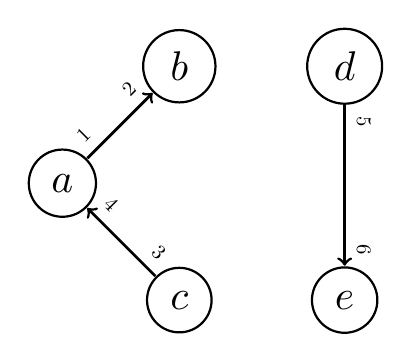
\begin{tikzpicture}[->,auto,node distance=1.4cm, thick,baseline=0]
			\tikzstyle{every node}=[shape=circle,draw=black,text=black,scale=1.5]
			\tikzstyle{every edge}=[line width=1pt,draw=black]
			
			\node         (1)                    {$a$};
			\node         (2) [above right of=1] {$b$};
			\node         (3) [below right of=1] {$c$};
			\node         (4) [right of=2]       {$d$};
			\node         (5) [right of=3]       {$e$};
			
			\draw (1) edge node [pos=0.15, sloped, above, draw=none, scale=0.5] {1} node [pos=0.85, sloped, above, draw=none, scale=0.5] {2} (2);
			\draw (3) edge node [pos=0.15, sloped, above, draw=none, scale=0.5] {3} node [pos=0.85, sloped, above, draw=none, scale=0.5] {4} (1);
			\draw (4) edge node [pos=0.1, sloped, above, draw=none, scale=0.5] {5} node [pos=0.9, sloped, above, draw=none, scale=0.5] {6} (5);
			\end{tikzpicture}
			
		\end{center}
		%\caption{ Example graph: ends of edges $\mathbf{Z}_{6} = 1,2,\;3,1,\;4,5$, vertex arrival times $\mathbf{T}_{5} = 1, 2, 3, 5, 6$, vertex counts $\mathbf{K}_{6} = 1, 2, \; 3, 3, \; 4, 5$, and degree counts $m_6(1) = 4, m_6(2) = 1$.}
	\end{figure}
\end{frame}

\begin{frame}
	\frametitle{Temporal networks}
	Number of vertices $K_n$ \\
	E.g. $K_6 = 5$
	\begin{figure}[H]
		\begin{center}
			% ,>=stealth',shorten >=1pt,
			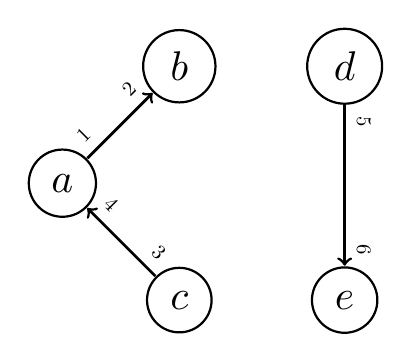
\begin{tikzpicture}[->,auto,node distance=1.4cm, thick,baseline=0]
			\tikzstyle{every node}=[shape=circle,draw=black,text=black,scale=1.5]
			\tikzstyle{every edge}=[line width=1pt,draw=black]
			
			\node         (1)                    {$a$};
			\node         (2) [above right of=1] {$b$};
			\node         (3) [below right of=1] {$c$};
			\node         (4) [right of=2]       {$d$};
			\node         (5) [right of=3]       {$e$};
			
			\draw (1) edge node [pos=0.15, sloped, above, draw=none, scale=0.5] {1} node [pos=0.85, sloped, above, draw=none, scale=0.5] {2} (2);
			\draw (3) edge node [pos=0.15, sloped, above, draw=none, scale=0.5] {3} node [pos=0.85, sloped, above, draw=none, scale=0.5] {4} (1);
			\draw (4) edge node [pos=0.1, sloped, above, draw=none, scale=0.5] {5} node [pos=0.9, sloped, above, draw=none, scale=0.5] {6} (5);
			\end{tikzpicture}
			
		\end{center}
		%\caption{ Example graph: ends of edges $\mathbf{Z}_{6} = 1,2,\;3,1,\;4,5$, vertex arrival times $\mathbf{T}_{5} = 1, 2, 3, 5, 6$, vertex counts $\mathbf{K}_{6} = 1, 2, \; 3, 3, \; 4, 5$, and degree counts $m_6(1) = 4, m_6(2) = 1$.}
	\end{figure}
\end{frame}

\begin{frame}
	\frametitle{Temporal networks}
	Arrival time of vertex $j$ is $T_j := \inf \{n: Z_n = j\}$ \\
	E.g. $T_e = 6$
	\begin{figure}[H]
		\begin{center}
			% ,>=stealth',shorten >=1pt,
			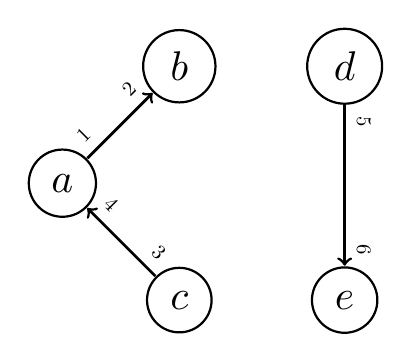
\begin{tikzpicture}[->,auto,node distance=1.4cm, thick,baseline=0]
			\tikzstyle{every node}=[shape=circle,draw=black,text=black,scale=1.5]
			\tikzstyle{every edge}=[line width=1pt,draw=black]
			
			\node         (1)                    {$a$};
			\node         (2) [above right of=1] {$b$};
			\node         (3) [below right of=1] {$c$};
			\node         (4) [right of=2]       {$d$};
			\node         (5) [right of=3]       {$e$};
			
			\draw (1) edge node [pos=0.15, sloped, above, draw=none, scale=0.5] {1} node [pos=0.85, sloped, above, draw=none, scale=0.5] {2} (2);
			\draw (3) edge node [pos=0.15, sloped, above, draw=none, scale=0.5] {3} node [pos=0.85, sloped, above, draw=none, scale=0.5] {4} (1);
			\draw (4) edge node [pos=0.1, sloped, above, draw=none, scale=0.5] {5} node [pos=0.9, sloped, above, draw=none, scale=0.5] {6} (5);
			\end{tikzpicture}
			
		\end{center}
		%\caption{ Example graph: ends of edges $\mathbf{Z}_{6} = 1,2,\;3,1,\;4,5$, vertex arrival times $\mathbf{T}_{5} = 1, 2, 3, 5, 6$, vertex counts $\mathbf{K}_{6} = 1, 2, \; 3, 3, \; 4, 5$, and degree counts $m_6(1) = 4, m_6(2) = 1$.}
	\end{figure}
\end{frame}

\begin{frame}
	\frametitle{Temporal networks}
	Degree of vertex $j$ is $d_{j,n}$ \\
	E.g. $d_{e,6} = 1$
	\begin{figure}[H]
		\begin{center}
			% ,>=stealth',shorten >=1pt,
			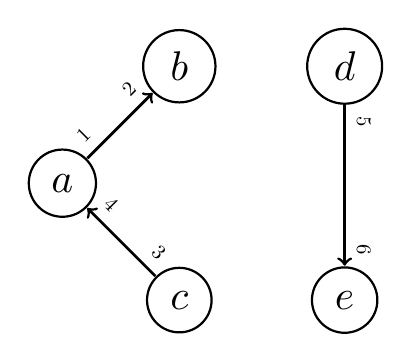
\begin{tikzpicture}[->,auto,node distance=1.4cm, thick,baseline=0]
			\tikzstyle{every node}=[shape=circle,draw=black,text=black,scale=1.5]
			\tikzstyle{every edge}=[line width=1pt,draw=black]
			
			\node         (1)                    {$a$};
			\node         (2) [above right of=1] {$b$};
			\node         (3) [below right of=1] {$c$};
			\node         (4) [right of=2]       {$d$};
			\node         (5) [right of=3]       {$e$};
			
			\draw (1) edge node [pos=0.15, sloped, above, draw=none, scale=0.5] {1} node [pos=0.85, sloped, above, draw=none, scale=0.5] {2} (2);
			\draw (3) edge node [pos=0.15, sloped, above, draw=none, scale=0.5] {3} node [pos=0.85, sloped, above, draw=none, scale=0.5] {4} (1);
			\draw (4) edge node [pos=0.1, sloped, above, draw=none, scale=0.5] {5} node [pos=0.9, sloped, above, draw=none, scale=0.5] {6} (5);
			\end{tikzpicture}
			
		\end{center}
		%\caption{ Example graph: ends of edges $\mathbf{Z}_{6} = 1,2,\;3,1,\;4,5$, vertex arrival times $\mathbf{T}_{5} = 1, 2, 3, 5, 6$, vertex counts $\mathbf{K}_{6} = 1, 2, \; 3, 3, \; 4, 5$, and degree counts $m_6(1) = 4, m_6(2) = 1$.}
	\end{figure}
\end{frame}

\begin{frame}
	\frametitle{Temporal networks}
	Degree counts $m_n(d) := |\{j: d_{j,n} = d\}|$ \\
	E.g. $m_6(1) = 4, m_6(2) = 1$
	\begin{figure}[H]
		\begin{center}
			% ,>=stealth',shorten >=1pt,
			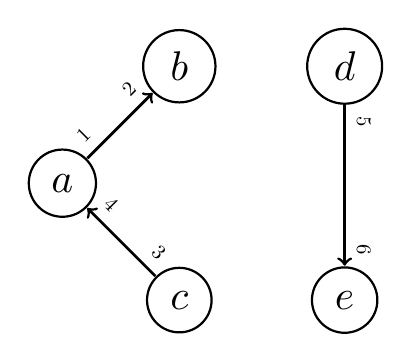
\begin{tikzpicture}[->,auto,node distance=1.4cm, thick,baseline=0]
			\tikzstyle{every node}=[shape=circle,draw=black,text=black,scale=1.5]
			\tikzstyle{every edge}=[line width=1pt,draw=black]
			
			\node         (1)                    {$a$};
			\node         (2) [above right of=1] {$b$};
			\node         (3) [below right of=1] {$c$};
			\node         (4) [right of=2]       {$d$};
			\node         (5) [right of=3]       {$e$};
			
			\draw (1) edge node [pos=0.15, sloped, above, draw=none, scale=0.5] {1} node [pos=0.85, sloped, above, draw=none, scale=0.5] {2} (2);
			\draw (3) edge node [pos=0.15, sloped, above, draw=none, scale=0.5] {3} node [pos=0.85, sloped, above, draw=none, scale=0.5] {4} (1);
			\draw (4) edge node [pos=0.1, sloped, above, draw=none, scale=0.5] {5} node [pos=0.9, sloped, above, draw=none, scale=0.5] {6} (5);
			\end{tikzpicture}
			
		\end{center}
		%\caption{ Example graph: ends of edges $\mathbf{Z}_{6} = 1,2,\;3,1,\;4,5$, vertex arrival times $\mathbf{T}_{5} = 1, 2, 3, 5, 6$, vertex counts $\mathbf{K}_{6} = 1, 2, \; 3, 3, \; 4, 5$, and degree counts $m_6(1) = 4, m_6(2) = 1$.}
	\end{figure}
\end{frame}



\subsection{Asymptotic properties}
\begin{frame}
	\frametitle{Sparsity}
	\begin{itemize}
		\item For a dense graph, $K_n = O(n^{1/2})$
		\item For a sparse graph,
		\begin{equation*}
			K_n = O(n^{1/(1+\sigma)})
		\end{equation*}
		for $0 \le \sigma < 1$
		\item Stack Overflow network likely sparse
	\end{itemize}
\end{frame}

\begin{frame}
	\frametitle{Power law degree distribution}
	A power law distribution of exponent $\eta$ on $\{1, 2, ...\}$ has
	\begin{equation*}
	p(d) \propto d^{-\eta} 
	\end{equation*}
	where $\eta > 1$.
	
	\pause
	The asymptotic degree distribution has \textbf{power law tail with exponent} $\eta > 1$ if
	\begin{align} 
	\label{eq:plaw}
	\frac{m_{n}(d)}{K_n} \xrightarrow[n\to\infty]{p} L(d)d^{-\eta} \;,
	\end{align}
	for slowly varying function $L(d)$.
	
	\vspace{20pt}
	\pause
	\small{A slowly varying function $L$ has the property ${\lim_{x\to\infty} L(rx)/L(x) = 1}$ for all ${r>0}$ \cite{bingham1989}.}
\end{frame}

\begin{frame}
	\frametitle{Power laws and sparsity}
	We have
	\begin{align*}
		K_n &= \sum_{d=1}^\infty m_n(d), \\
		n &= \sum_{d=1}^\infty d\, m_n(d).
	\end{align*}
\end{frame}

\begin{frame}
	\frametitle{Power laws and sparsity}
	Suppose $m_n(d)$ is power law distributed
	\begin{align*}
	K_n &= C \sum_{d=1}^n d^{-\eta}, \\
	n &= C \sum_{d=1}^n d^{-\eta + 1} = K_n \, \frac{\sum_{d=1}^n d^{-\eta + 1}}{\sum_{d=1}^n d^{-\eta}}.
	\end{align*}
\end{frame}

\begin{frame}
	\frametitle{Power laws and sparsity}
	Letting $n\to \infty$ in
	\begin{equation*}
		\frac{K_n}{n} = \frac{\sum_{d=1}^n d^{-\eta}}{\sum_{d=1}^n d^{-\eta + 1}}
	\end{equation*}
	we see $K_n = O(n)$ if $\eta > 2$, $K_n = o(n)$ if $\eta \in (1, 2]$.
	\vspace{40pt}
	\pause
	
	\textbf{Summary}
	
	For sparse graphs, $\sigma=0 \leftrightarrow \eta > 2$ and $\sigma > 0 \leftrightarrow \eta \in (1,2]$.
\end{frame}

\subsection{Empirical study}
\begin{frame}
	\frametitle{Empirical study}
	\textbf{SNAP datasets} \cite{snapnets}
	\begin{table}[b]
		% \vspace*{-\baselineskip}
		\label{tab:datasets}
		\begin{center}
			\begin{tabular}{lll}
				Dataset                 & \# of vertices   & \# of edges    \\
				\hline
				Ask Ubuntu    & 159,316   & 964,437    \\
				UCI social network   & 1,899     & 20,296     \\
				EU email        & 986       & 332,334    \\
				Math Overflow & 24,818    & 506,550    \\
				Stack Overflow           & 2,601,977 & 63,497,050 \\
				Super User    & 194,085   & 1,443,339  \\
				Wikipedia talk pages    & 1,140,149 & 7,833,140 \\
			\end{tabular}
		\end{center}
	\end{table}
	
\end{frame}

\begin{frame}
	\frametitle{Ask Ubuntu arrival process}
	\begin{figure}[h]
		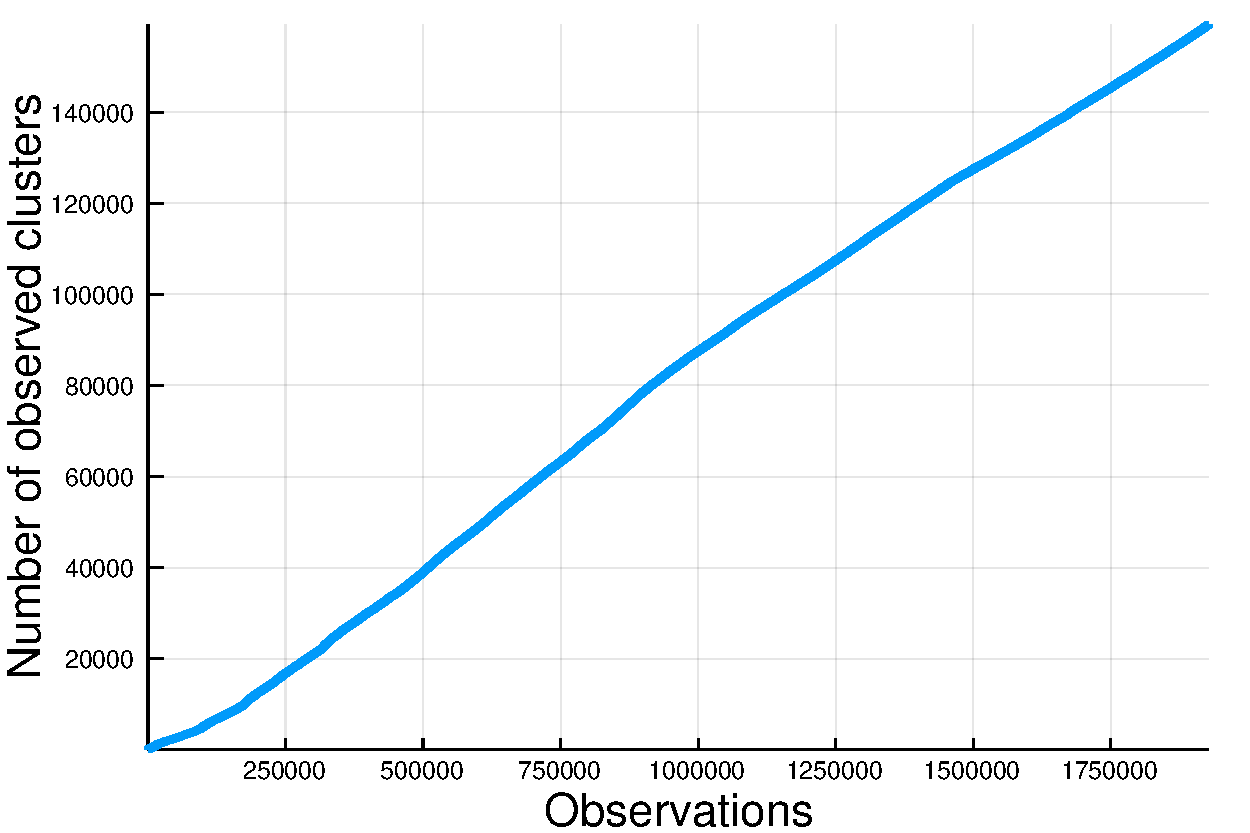
\includegraphics[width=0.8\textwidth]{fig/arrival_times_askubuntu.pdf}
	\end{figure}
	
\end{frame}

\begin{frame}
	\frametitle{Stack Overflow arrival process}
	\begin{figure}[h]
		\includegraphics[width=0.8\textwidth]{fig/arrival_times_stackoverflow.pdf}
	\end{figure}
	
\end{frame}

\begin{frame}
	\frametitle{UCI social network arrival process}
	\begin{figure}[h]
		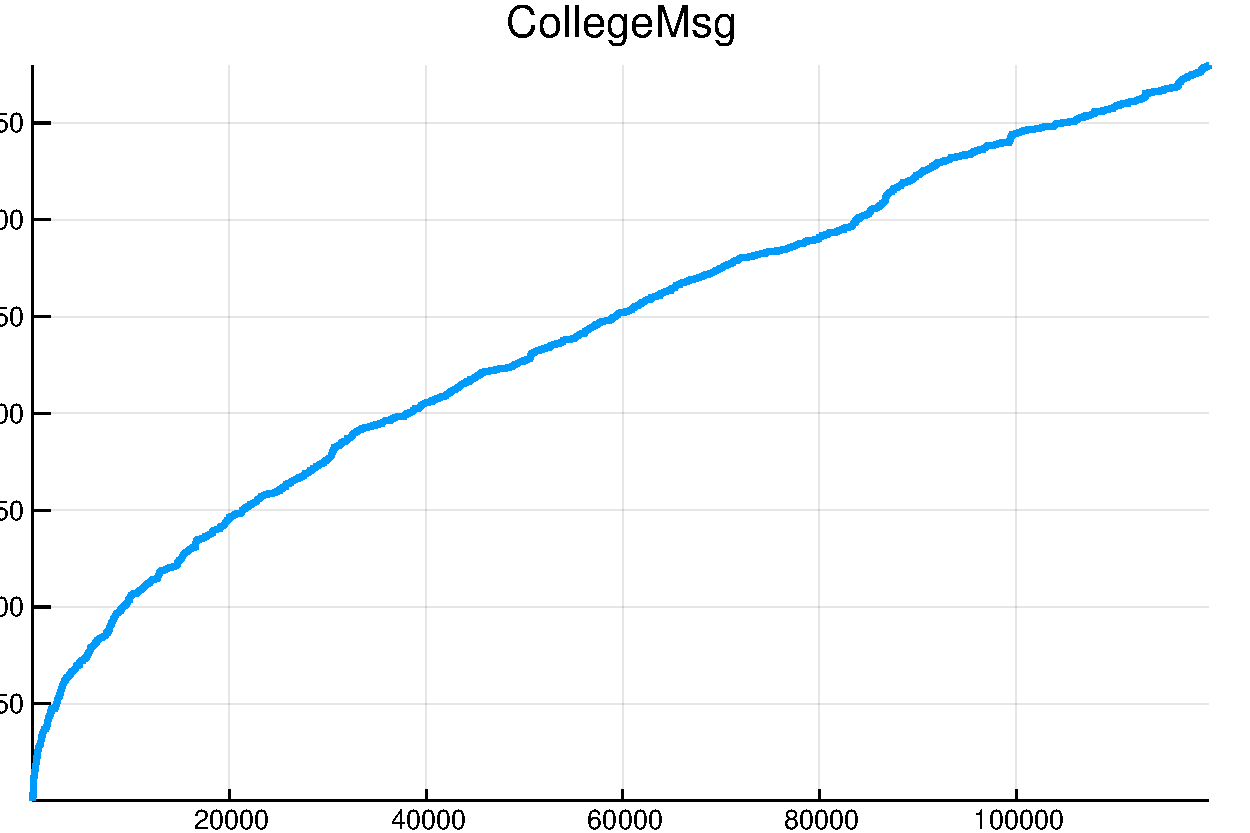
\includegraphics[width=0.8\textwidth]{fig/arrival_times_CollegeMsg.pdf}
	\end{figure}
	
\end{frame}

\begin{frame}
	\frametitle{Ask Ubuntu degree distribution}
	\begin{figure}[h]
		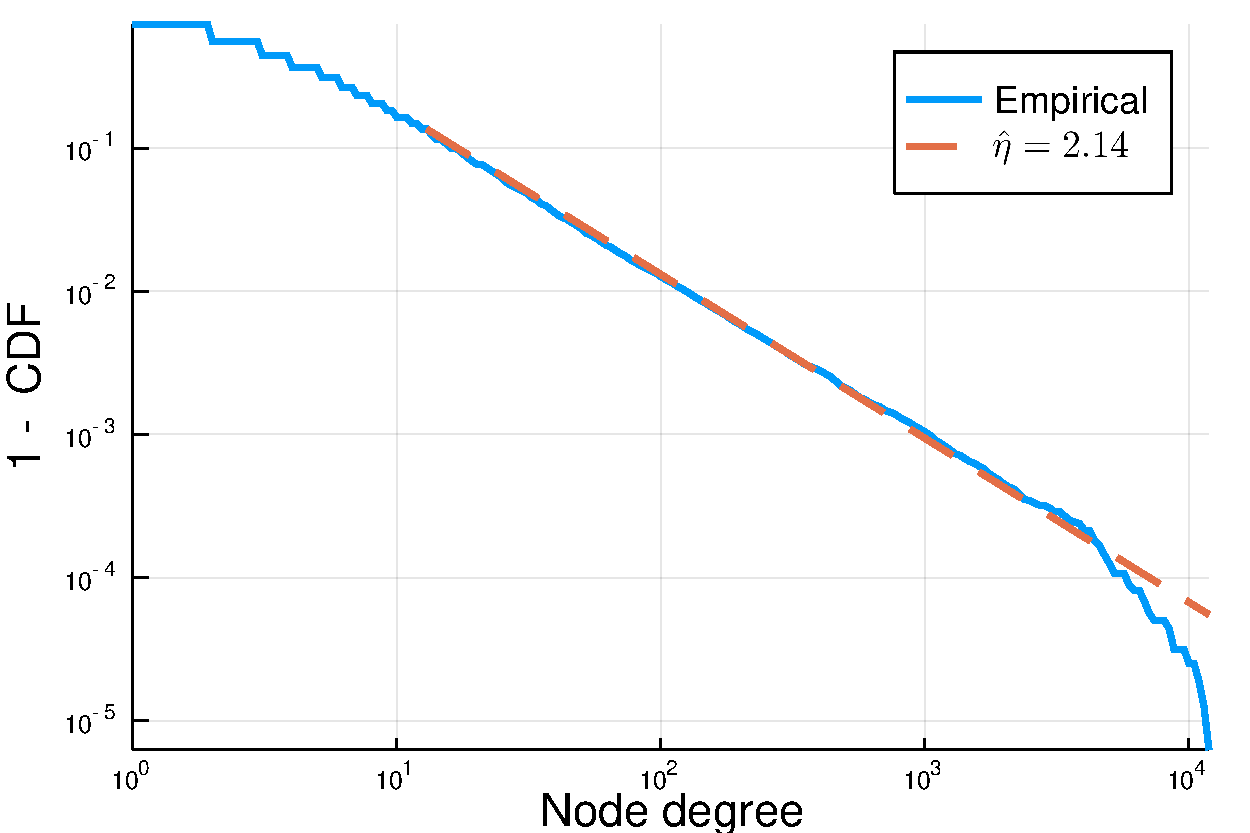
\includegraphics[width=0.8\textwidth]{fig/nodes_degre_power_law_askubuntu.pdf}
	\end{figure}
	
	Estimation used technique of \cite{clauset}
	
\end{frame}

\begin{frame}
	\frametitle{Todo}
	\begin{itemize}
		\item Recompile the images with better labels on the axes
		\item Estimate $\sigma$ by linear regression
	\end{itemize}
	
\end{frame}

\subsection{Models}
\begin{frame}
	\frametitle{Models}
	\begin{itemize}
		\item Vertex exchangeable models do not give sparsity \cite{aldous1981} \cite{hoover1979}
		\item Exchangeable point process models \cite{caronfox} have an independent notion of time
		\item \textbf{Preferential attachment models} \cite{barabasi1999}
		\item \textbf{Edge exchangeable models} \cite{CraneDempsey2017} \cite{cai2016}
	\end{itemize}
\end{frame}

\begin{frame}
	\frametitle{Yule-Simon Process}
	Parameter $\beta \in (0, 1)$.
	\vspace{15pt}
	
	Arrivals
	\begin{align*}
	T_{j+1} - T_{j} \simiid \text{Geom}\left( \beta \right)
	\end{align*}
	Size-biased reinforcement
	\begin{align*} 
	\ee_{n+1} | \bfee_{n}, \bfT &= \begin{cases}\begin{aligned}
	K_{n+1} & \text{ w.p. } 1 && \text{if } n+1 = T_{K_{n+1}} \\
	j &\text{ w.p.} \propto d_{j,n} && \text{otherwise} 
	\end{aligned}\end{cases}
	\label{eq:ys}
	\end{align*}
\end{frame}

\begin{frame}
	\frametitle{Yule-Simon Process}
	Asymptotic power law degree distribution with
	\begin{equation*}
		\eta = 1 + \frac{1}{1-\beta} > 2
	\end{equation*}
	and $K_n = O(n)$
\end{frame}

\begin{frame}
	\frametitle{Pitman-Yor Process}
	Parameters $\tau \in (0, 1), \theta > -\tau$.
	\vspace{15pt}
	
	Urn process
	\begin{align*} 
	\ee_{n+1} | \bfee_{n} &= \begin{cases}\begin{aligned}
	K_{n+1} & \text{ w.p. } \frac{\theta + K_n \tau}{n + \theta}  \\
	& \\
	j &\text{ w.p. } \frac{d_{j,n} - \tau}{\theta + n} 
	\end{aligned}\end{cases}
	\label{eq:pyp2}
	\end{align*}
\end{frame}

\begin{frame}
	\frametitle{Pitman-Yor Process}
	Asymptotic power law degree distribution with
	\begin{equation*}
		\eta = 1 + \tau \in (1, 2)
	\end{equation*}
	and $K_n = o(n)$
\end{frame}


\begin{frame}
	\frametitle{Edge exchangeable models \cite{cai2016}, \cite{CraneDempsey2017}}
	``The probability of all orderings of edge arrivals is the same''
	
	\vspace{20pt}
	
	$\eta \in (1,2)$
	
	$\exists$ a class of models that includes (some) edge exchangeable models, but also YS and admits all the $\eta$s
	
\end{frame}

\begin{frame}
	\frametitle{Rewriting the Pitman-Yor Process}
	Parameters $\tau \in (0, 1), \theta > -\tau$.
	\vspace{15pt}
	
	Arrivals
	\begin{align*}
	\bbP(T_{j+1} - T_j > t \mid T_j) = \prod_{i=1}^{t} \frac{T_j + t - j \tau}{T_j + t + \theta}
	\end{align*}
	Size-biased reinforcement
	\begin{align*} 
	\ee_{n+1} | \bfee_{n}, \bfT &= \begin{cases}\begin{aligned}
	K_{n+1} & \text{ w.p. } 1 && \text{if } n+1 = T_{K_{n+1}} \\
	j &\text{ w.p.} \propto (d_{j,n} - \tau) && \text{otherwise} 
	\end{aligned}\end{cases}
	\end{align*}
\end{frame}

\begin{frame}
	\frametitle{Beta Neutral-to-the-left Process \cite{Bloem2017}}
	Parameters $\alpha \in (-\infty, 1)$ and $\Lambda_\phi$ a law on $\mathbb{N}^\infty$.
	\vspace{15pt}
	
	Arrivals
	\begin{align*}
	\bfT \sim \Lambda_\phi
	\end{align*}
	Size-biased reinforcement
	\begin{align*} 
	\ee_{n+1} | \bfee_{n}, \bfT &= \begin{cases}\begin{aligned}
	K_{n+1} & \text{ w.p. } 1 && \text{if } n+1 = T_{K_{n+1}} \\
	j &\text{ w.p.} \propto (d_{j,n} - \alpha) && \text{otherwise} 
	\end{aligned}\end{cases}
	\label{eq:bntl}
	\end{align*}
\end{frame}

\begin{frame}
	\frametitle{Relationship with other model classes}
	\begin{figure}[H]
		\begin{center}
			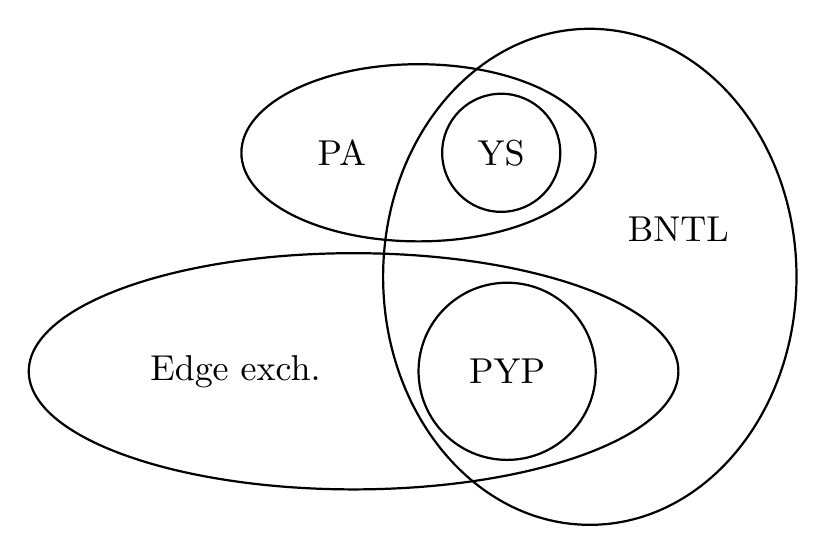
\begin{tikzpicture}[->,auto,node distance=3.6cm, thick,baseline=0,scale=0.75]
			
			\tikzstyle{every node}=[scale=1.3]
			
			\def\pyp{(-0.9,-0.2) coordinate (a) circle (1.5cm)}
			\def\ys{(-1,3.5) coordinate (b)  circle (1cm)}
			\def\ex{(-3.5,-0.2) coordinate (c) ellipse (5.5cm and 2cm)}
			\def\pa{(-2.4,3.5) coordinate (d) ellipse (3cm and 1.5cm)}
			\def\bntl{(0.5,1.4) coordinate (e) ellipse (3.5cm and 4.2cm)}
			
			\draw \pyp  node {PYP};
			\draw \ys node {YS};
			\draw \ex;
			\draw node at (-5.5,-0.2) {Edge exch.};
			\draw \pa;
			\draw node at (-3.7, 3.5) {PA};
			\draw \bntl;
			\draw node at (2,2.2) {BNTL};
			\end{tikzpicture}
		\end{center}
	\end{figure}
\end{frame}

\begin{frame}
	\frametitle{Hierarchical representation of BNTL process}
	Arrivals
	\begin{equation*}
	\bfT \sim \Lambda_\phi
	\end{equation*}
	Latent sociabilities
	\begin{equation*}
		\Psi_j | T_j \sim \text{Beta}(1-\alpha,T_j-1-(j-1)\alpha) \text{ for } j\geq 1
	\end{equation*}
	Left-neutral resampling probabilities
	\begin{align*}
		P_{j,k+1} = 
		\begin{cases}
		P_{j,k}(1-\Psi_{k+1}), & j \in \{1,\dots,k\} \\
		\Psi_{k+1}, & j = k+1
		\end{cases}
	\end{align*}
	Sampling rule
	\begin{align*} 
		\ee_{n+1} | \mathbf{P}_{K_n}, \bfT &= \begin{cases}\begin{aligned}
		K_{n+1} & \text{ w.p. } 1 && \text{if } n+1 = T_{K_{n+1}} \\
		j &\text{ w.p. } P_{j, K_n} && \text{otherwise} 
		\end{aligned}\end{cases}
	\end{align*}
\end{frame}

\begin{frame}
	\frametitle{BNTL properties}
	\begin{itemize}
		\item Collapsed sampler
		\item Latent representation
		\item But \textit{not} from de Finetti -- latents change with $K_n$
	\end{itemize}
\end{frame}


\section{Sampling and inference}
\subsection{Preliminaries}
\begin{frame}
	\frametitle{Sampling and inference}
	\begin{itemize}
		\item Sampling posterior on latents
		\item Point estimation of latents
		\item Sampling predictive distribution
	\end{itemize}
\end{frame}

\begin{frame}
	\frametitle{Sampling and inference}
	\begin{itemize}
		\item Sampling posterior on latents \textbf{Condition on what?}
		\item Point estimation of latents 
		\item Sampling predictive distribution
	\end{itemize}
\end{frame}

\begin{frame}
	\frametitle{Observation cases}
	\begin{center}
		\begin{tabular}{ll}
			\textbf{Observation} & \textbf{Unobserved variables} \\
			\hline
			End of edge sequence $\bfee_n$ & $\alpha,\phi,\bfPsi_{K_n}$ \\
			Vertex arrival-ordered graph & $\alpha,\phi,\bfPsi_{K_n}, \bfT_{K_n}$ \\
			Unlabeled graph & $\alpha,\phi,\bfPsi_{K_n},\bfT_{K_n},\sigma [K_n]$
		\end{tabular}
	\end{center}
\end{frame}

\subsection{Gibbs sampler}
\begin{frame}
\frametitle{Sampling $\bfPsi$}

If $\bfee_n$ or $d_{K_n}$ observed
\begin{align*}
	p_{\alpha, \phi}(\bfPsi_{K_n}, \bfee_n | \bfT_{K_n}, \bfd_{K_n}) &\propto \prod_{j=1}^{K_n} &&\Psi_j ^{ - \alpha} (1-\Psi_j)^{T_j - (j-1)\alpha - 1} \\
	&&&\cdot \prod_{j=1}^{K_n} \Psi_j^{d_{j,n}-1}(1-\Psi_j)^{\bar{d}_{j-1,n} - T_j}\\
	&\propto \prod_{j=1}^{K_n} &&\Psi_j ^{d_{j,n} - \alpha -1} (1-\Psi_j)^{\bar{d}_{j-1,n} - (j-1)\alpha - 1}
\end{align*}
where
\begin{equation*}
\bar{d}_{j,n} = \sum_{i=1}^j d_{j,n}.
\end{equation*}

\end{frame}

\begin{frame}
	\frametitle{Sampling $\bfPsi$}
	Spot a closed form for $\bfPsi$
	\begin{equation*}
	\Psi_j \mid \bfee_n, \bfPsi_{\setminus j} \sim \text{Beta}(d_{j,n} - \alpha, \bar{d}_{j-1,n} - (j-1)\alpha) \;,
	\end{equation*}
	
	\begin{itemize}
		\item For fixed $\alpha$, we have our posterior
		\item Learning other variables, we have a Gibbs update
	\end{itemize}
\end{frame}

\begin{frame}
	\frametitle{Sampling $\alpha, \phi$}
	\begin{itemize}
		\item Place priors on $\alpha, \phi$
		\item Left with one-dimensional unnormalized density for $\alpha$ and MCMC is applicable
		\item For $\phi$, depends on $\Lambda_\phi$. Our experiments used conjugacy or slice sampling.
	\end{itemize}

\end{frame}

\begin{frame}
	\frametitle{Sampling $\bfT$}
	Assume
	\begin{align*}
	\aDist^{\phi}(\bfT_k) = \delta_{T_1}(1) \prod_{j=2}^k \aDist_j^{\phi}(\Delta_j | T_{j-1}) \;,
	\end{align*}
	Support of $T_j - T_{j-1} | T_{\backslash j}$ is
	\begin{equation*}
		\{ 1, ..., \min(T_{j+1} - T_{j-1} - 1, \bar{d}_{j-1} - T_{j-1} + 1)  \}
	\end{equation*}
	and we can compute each probability
	\begin{align*}
		p_{\alpha, \phi}(T_j - T_{j-1} = s | \bfT_{\backslash j} , \bfd_{K}) \propto &\  \Lambda_j^\phi(s|T_{j-1})\Lambda_{j+1}^\phi (T_{j+1}-T_{j-1} - s) \\
		&\cdot \binom{\bar{d}_j - T_{j-1} - s}{d_j - 1}
	\end{align*}
	and sample.
\end{frame}

\begin{frame}
	\frametitle{Sampling $\sigma[K_n]$}\

	\begin{itemize} 
	\item Use Metropolis-Hastings with swap proposal $\sigma_j \leftrightarrow \sigma_{j+1}$
	
	\item Ratio of joints can be easily computed in terms of $\Gamma$ function.
	\end{itemize}
\end{frame}

\subsection{Point estimation}
\begin{frame}
	\frametitle{Point estimation}
	\begin{itemize} 
	
		\item Factorization $p_{\alpha, \phi}(\bfee_n) = p_\alpha (\bfee_n | \bfT_{K_n})\Lambda_\phi(\bfT_{K_n})$ 

		\item Learn $\alpha$ separately from $\phi$ using standard optimization (low dimensional)
	
		\item We have explicit formulae for MLE/MAP estimates for $\bfPsi$
	\end{itemize}
\end{frame}

\section{Experiments}
\subsection{Inference}
\begin{frame}
	\frametitle{Synthetic data}
	\begin{itemize}
		\item Simulate 500 edges from the prior with fixed $\alpha$, $\Lambda_\phi$ 
		\item Either $\PYP$ or $\Geom$
		\item Observe final snapshot of the graph only
	\end{itemize}
\end{frame}

\begin{frame}
	\frametitle{Gibbs sampler results}
	\begin{table}[h]
		%  \caption{Results of Gibbs sampling experiments on synthetic data $(\alpha^* = 0.75)$. The top four rows show results from each of four different BNTL models fit to a synthetic graph with 500 edges generated by the coupled $\PYP$ BNTL model; the bottom four rows show the same BNTL models fit to a synthetic graph with $\Geom(0.25)$-distributed interarrivals.}
		\label{tab:ess}
		\vspace*{-0.75\baselineskip}
		\begin{center}
			\resizebox{1.0\textwidth}{!}{
				\begin{tabular}{lllll}
					Gen. arrival distn. & Inference model & $|\hat{\alpha} - \alpha^*|$ & $|\mathbf{\hat{S}} - \mathbf{S^*}|$ & Pred. log-lik.  \\
					\hline
					$\PYP(1.0,0.75)$ &  $(\tau,\PYP(\theta,\tau))$ &  \textbf{0.046 $\pm$ 0.002}  &  \textbf{28.5 $\pm$ 0.7}  & -\textbf{2637.0 $\pm$ 0.1}  \\ 
					
					$\PYP(1.0,0.75)$  &  $(\alpha,\Geom(\beta))$  &  {0.049 $\pm$ 0.004}  &  66.8 $\pm$ 1.2  & -2660.5 $\pm$ 0.7  \\ 
					\hline
					
					$\Geom(0.25)$ & $(\tau,\PYP(\theta,\tau))$ &  0.086 $\pm$ 0.002  &  56.6 $\pm$ 1.3  & -2386.8 $\pm$ 0.1  \\  
					
					$\Geom(0.25)$ & $(\alpha,\Geom(\beta))$ &  \textbf{0.043 $\pm$ 0.003}  &  \textbf{24.8 $\pm$ 0.8}  & -\textbf{2382.6 $\pm$ 0.2}  \\ 
					
					\end{tabular}
					}
				\end{center}
			\end{table}
			
where $\mathbf{S} := \frac{1}{K_n - 1} \sum_{j>1} (\bar{d}_{j-1} - T_j)$
\end{frame}

\subsection{Scalability of Gibbs sampler}
\begin{frame}
	\frametitle{Scalability of Gibbs sampler}
	\begin{itemize}
		\item Do we learn from all data?
		\item How does performance scale?
	\end{itemize}
	\pause
	
	\begin{table}[t]
		\label{tab:ess:scale:n}
		\vspace*{-0.25\baselineskip}
		\begin{center}
			%  \resizebox{0.6\textwidth}{!}{
			\begin{tabular}{l  ll}
				& $n=200$ &  $n=20000$ \\ 
				\hline
				$|\hat{\alpha} - \alpha^*|$ & 0.12 $\pm$ 0.01 &  0.01 $\pm$ 0.00 \\ 
				
				$|\hat{\beta} - \beta^*|$ &  0.02 $\pm$ 0.00  &    0.00 $\pm$ 0.00  \\ 
				
				ESS &  0.90 $\pm$ 0.04  &   0.75 $\pm$ 0.08  \\  
				
				Runtime (s) &  21 $\pm$ 0   &  2267 $\pm$ 2  \\ 
				
			\end{tabular}
			%}
		\end{center}
	\end{table}
	\begin{itemize}
		\item Most expensive Gibss update is for $\bfT$
	\end{itemize}
\end{frame}

\subsection{Large scale real data experiments}
\begin{frame}
	\frametitle{Large scale real data experiments}
	\begin{itemize}
		\item MLE point estimation for SNAP datasets
		\item Predictive log-likelihood
	\end{itemize}
	
\end{frame}


\begin{frame}
	\frametitle{MLEs for SNAP datasets}
	$\PYP$ parameter estimates vary coupled and uncoupled
	\begin{table}[!ht]
		\begin{center}
			\color{lightgray}{
			\resizebox{1.05\textwidth}{!}{
				\begin{tabular}{llll | lllllll}
					\multirow{2}{*}{Dataset} & \multicolumn{3}{c}{\color{black}{Coupled $\PYP(\theta,\alpha)$}}  & &  \multicolumn{2}{c}{\color{black}{Uncoupled $\PYP(\theta,\tau)$}} &  & \multicolumn{3}{c}{$\Geom(\geom)$}                             \\
					\cline{2-4} \cline{6-7} \cline{9-11}
					& \color{black}{$(\hat{\theta},\hat{\alpha})$} & $\hat{\eta}$           & Pred. l-l.            & \color{black}{$\hat{\alpha}$}    & \color{black}{$(\hat{\theta},\hat{\tau})$} & Pred. l-l.     &     & $\hat{\beta}$  & $\hat{\eta}$   & Pred. l-l.                             \\
					\hline
					Ask Ubuntu  & \color{black}{(18080, 0.25)} & 1.25   & -3.707e6              & \color{black}{-2.54}            & \color{black}{(-0.99, 0.99)}    & -3.678e6  &   &  0.083 & 2.32    & \textbf{-3.678e6}                         \\
					UCI social network & (320.4, 4.4e-11) & --   & -1.600e5            & -4.98             & (5.50, 0.52)     & \textbf{-1.595e6}   &  & 0.016  & 2.10  & -1.596e5                    \\
					EU email   & (113.6, 2.5e-14)  & --    & \textbf{-8.06e5}              & -1.86              & (113.6, 9.2e-10)      & \textbf{-8.06e5}  &   & 0.001  & 2.00   & -8.07e5                     \\
					Math Overflow & (2575, 0.15) & 1.15  & -1.685e6              & -6.62           & (-0.97, 0.997)    & -1.670e6 &    & 0.025  & 2.19   & \textbf{-1.670e6}                \\
					Stack Overflow & \color{black}{(297600, 0.11)} & 1.11 & -3.358e8             & \color{black}{-8.94}            & \color{black}{(-1.0, 1.0)}      &  -3.333e8  &    &  0.020  & 2.21   & \textbf{-3.333e8}                 \\
					Super User  & (20640, 0.24) & 1.24  & -5.855e6            & -4.19          & (-0.996, 1.0)      &  \textbf{-5.775e6}   &  & 0.067 & 2.37    & -5.775e6              \\
					Wikipedia talk pages  & (14870, 0.54) & 1.54  & -3.074e7          & -0.25            & (-1.0, 1.0)   & \textbf{-3.066e7}  &   & 0.073  & 2.10   & -3.066e7                   
				\end{tabular}
			}}
		\end{center}
		\vspace*{-\baselineskip}
	\end{table}
\end{frame}

\begin{frame}
	\frametitle{MLEs for SNAP datasets}
	Edge exchangeable models likely misspecified 
	\begin{table}[!ht]
		\begin{center}
			\color{lightgray}{
				\resizebox{1.05\textwidth}{!}{
					\begin{tabular}{llll | lllllll}
						\multirow{2}{*}{Dataset} & \multicolumn{3}{c}{Coupled $\PYP(\theta,\alpha)$}  & &  \multicolumn{2}{c}{Uncoupled $\PYP(\theta,\tau)$} &  & \multicolumn{3}{c}{\color{black}{$\Geom(\geom)$}}                             \\
						\cline{2-4} \cline{6-7} \cline{9-11}
						& $(\hat{\theta},\hat{\alpha})$ & $\hat{\eta}$           & Pred. l-l.            & $\hat{\alpha}$    & $(\hat{\theta},\hat{\tau})$ & Pred. l-l.     &     & $\hat{\beta}$  & \color{black}{$\hat{\eta}$}   & Pred. l-l.                             \\
						\hline
						\color{black}{Ask Ubuntu}  & (18080, 0.25) & 1.25   & -3.707e6              & -2.54            & (-0.99, 0.99)    & -3.678e6  &   &  0.083 & \color{black}{2.32}    & \textbf{-3.678e6}                         \\
						UCI social network & (320.4, 4.4e-11) & --   & -1.600e5            & -4.98             & (5.50, 0.52)     & \textbf{-1.595e6}   &  & 0.016  & 2.10  & -1.596e5                    \\
						EU email   & (113.6, 2.5e-14)  & --    & \textbf{-8.06e5}              & -1.86              & (113.6, 9.2e-10)      & \textbf{-8.06e5}  &   & 0.001  & 2.00   & -8.07e5                     \\
						Math Overflow & (2575, 0.15) & 1.15  & -1.685e6              & -6.62           & (-0.97, 0.997)    & -1.670e6 &    & 0.025  & 2.19   & \textbf{-1.670e6}                \\
						\color{black}{Stack Overflow} & (297600, 0.11) & 1.11 & -3.358e8             & -8.94            & (-1.0, 1.0)      &  -3.333e8  &    &  0.020  & \color{black}{2.21}   & \textbf{-3.333e8}                 \\
						Super User  & (20640, 0.24) & 1.24  & -5.855e6            & -4.19          & (-0.996, 1.0)      &  \textbf{-5.775e6}   &  & 0.067 & 2.37    & -5.775e6              \\
						Wikipedia talk pages  & (14870, 0.54) & 1.54  & -3.074e7          & -0.25            & (-1.0, 1.0)   & \textbf{-3.066e7}  &   & 0.073  & 2.10   & -3.066e7                   
					\end{tabular}
				}}
			\end{center}
			\vspace*{-\baselineskip}
		\end{table}
	\end{frame}
	
\begin{frame}
	\frametitle{MLEs for SNAP datasets}
	Though better than $\Geom$ for some datasets
	\begin{table}[!ht]
		\begin{center}
			\color{lightgray}{
				\resizebox{1.05\textwidth}{!}{
					\begin{tabular}{llll | lllllll}
						\multirow{2}{*}{Dataset} & \multicolumn{3}{c}{Coupled $\PYP(\theta,\alpha)$}  & &  \multicolumn{2}{c}{Uncoupled $\PYP(\theta,\tau)$} &  & \multicolumn{3}{c}{$\Geom(\geom)$}                             \\
						\cline{2-4} \cline{6-7} \cline{9-11}
						& $(\hat{\theta},\hat{\alpha})$ & $\hat{\eta}$           & Pred. l-l.            & $\hat{\alpha}$    & $(\hat{\theta},\hat{\tau})$ & Pred. l-l.     &     & $\hat{\beta}$  & $\hat{\eta}$   & Pred. l-l.                             \\
						\hline
						Ask Ubuntu  & (18080, 0.25) & 1.25   & -3.707e6              & -2.54            & (-0.99, 0.99)    & -3.678e6  &   &  0.083 & 2.32    & \textbf{-3.678e6}                         \\
						UCI social network & (320.4, 4.4e-11) & --   & -1.600e5            & -4.98             & (5.50, 0.52)     & \textbf{-1.595e6}   &  & 0.016  & 2.10  & -1.596e5                    \\
						\color{black}{EU email}   & \color{black}{(113.6, 2.5e-14)}  & --    & \color{black}{\textbf{-8.06e5}}              & \color{black}{-1.86}              & \color{black}{(113.6, 9.2e-10)}      & \color{black}{\textbf{-8.06e5}}  &   & \color{black}{0.001}  & \color{black}{2.00}   & \color{black}{-8.07e5}                     \\
						Math Overflow & (2575, 0.15) & 1.15  & -1.685e6              & -6.62           & (-0.97, 0.997)    & -1.670e6 &    & 0.025  & 2.19   & \textbf{-1.670e6}                \\
						Stack Overflow & (297600, 0.11) & 1.11 & -3.358e8             & -8.94            & (-1.0, 1.0)      &  -3.333e8  &    &  0.020  & 2.21   & \textbf{-3.333e8}                 \\
						Super User  & (20640, 0.24) & 1.24  & -5.855e6            & -4.19          & (-0.996, 1.0)      &  \textbf{-5.775e6}   &  & 0.067 & 2.37    & -5.775e6              \\
						Wikipedia talk pages  & (14870, 0.54) & 1.54  & -3.074e7          & -0.25            & (-1.0, 1.0)   & \textbf{-3.066e7}  &   & 0.073  & 2.10   & -3.066e7                   
					\end{tabular}
				}}
			\end{center}
			\vspace*{-\baselineskip}
		\end{table}
	\end{frame}
	
\begin{frame}
	\frametitle{MLEs for SNAP datasets}
	These datasets may lack sparsity
	\begin{table}[!ht]
		\begin{center}
			\color{lightgray}{
				\resizebox{1.05\textwidth}{!}{
					\begin{tabular}{llll | lllllll}
						\multirow{2}{*}{Dataset} & \multicolumn{3}{c}{\color{black}{Coupled $\PYP(\theta,\alpha)$}}  & &  \multicolumn{2}{c}{\color{black}{Uncoupled $\PYP(\theta,\tau)$}} &  & \multicolumn{3}{c}{\color{black}{$\Geom(\geom)$}}                             \\
						\cline{2-4} \cline{6-7} \cline{9-11}
						& $(\hat{\theta},\hat{\alpha})$ & \color{black}{$\hat{\eta}$}           & Pred. l-l.            & $\hat{\alpha}$    & $(\hat{\theta},\hat{\tau})$ & Pred. l-l.     &     & $\hat{\beta}$  & $\hat{\eta}$   & Pred. l-l.                             \\
						\hline
						Ask Ubuntu  & (18080, 0.25) & 1.25   & -3.707e6              & -2.54            & (-0.99, 0.99)    & -3.678e6  &   &  0.083 & 2.32    & \textbf{-3.678e6}                         \\
						\color{black}{UCI social network} & \color{black}{(320.4, 4.4e-11)} & \color{black}{--}   & -1.600e5            & -4.98             & (5.50, 0.52)     & \textbf{-1.595e6}   &  & 0.016  & 2.10  & -1.596e5                    \\
						\color{black}{EU email}   & \color{black}{(113.6, 2.5e-14)}  & \color{black}{--}    & \textbf{-8.06e5}              & -1.86              & (113.6, 9.2e-10)      & \textbf{-8.06e5}  &   & 0.001  & 2.00   & -8.07e5                     \\
						Math Overflow & (2575, 0.15) & 1.15  & -1.685e6              & -6.62           & (-0.97, 0.997)    & -1.670e6 &    & 0.025  & 2.19   & \textbf{-1.670e6}                \\
						Stack Overflow & (297600, 0.11) & 1.11 & -3.358e8             & -8.94            & (-1.0, 1.0)      &  -3.333e8  &    &  0.020  & 2.21   & \textbf{-3.333e8}                 \\
						Super User  & (20640, 0.24) & 1.24  & -5.855e6            & -4.19          & (-0.996, 1.0)      &  \textbf{-5.775e6}   &  & 0.067 & 2.37    & -5.775e6              \\
						Wikipedia talk pages  & (14870, 0.54) & 1.54  & -3.074e7          & -0.25            & (-1.0, 1.0)   & \textbf{-3.066e7}  &   & 0.073  & 2.10   & -3.066e7                   
					\end{tabular}
				}}
			\end{center}
			\vspace*{-\baselineskip}
		\end{table}
	\end{frame}
	
%\begin{frame}
%	\frametitle{MLEs for SNAP datasets}
%	Though not for all datasets
%	\begin{table}[!ht]
%		\begin{center}
%			\color{lightgray}{
%				\resizebox{1.05\textwidth}{!}{
%					\begin{tabular}{llll | lllllll}
%						\multirow{2}{*}{Dataset} & \multicolumn{3}{c}{Coupled $\PYP(\theta,\alpha)$}  & &  \multicolumn{2}{c}{Uncoupled $\PYP(\theta,\tau)$} &  & \multicolumn{3}{c}{$\Geom(\geom)$}                             \\
%						\cline{2-4} \cline{6-7} \cline{9-11}
%						& $(\hat{\theta},\hat{\alpha})$ & $\hat{\eta}$           & Pred. l-l.            & $\hat{\alpha}$    & $(\hat{\theta},\hat{\tau})$ & Pred. l-l.     &     & $\hat{\beta}$  & $\hat{\eta}$   & Pred. l-l.                             \\
%						\hline
%						Ask Ubuntu  & (18080, 0.25) & 1.25   & -3.707e6              & -2.54            & (-0.99, 0.99)    & -3.678e6  &   &  0.083 & 2.32    & \textbf{-3.678e6}                         \\
%						UCI social network & (320.4, 4.4e-11) & --   & -1.600e5            & -4.98             & (5.50, 0.52)     & \textbf{-1.595e6}   &  & 0.016  & 2.10  & -1.596e5                    \\
%						EU email   & (113.6, 2.5e-14)  & --    & \textbf{-8.06e5}              & -1.86              & (113.6, 9.2e-10)      & \textbf{-8.06e5}  &   & 0.001  & 2.00   & -8.07e5                     \\
%						Math Overflow & (2575, 0.15) & 1.15  & -1.685e6              & -6.62           & (-0.97, 0.997)    & -1.670e6 &    & 0.025  & 2.19   & \textbf{-1.670e6}                \\
%						Stack Overflow & (297600, 0.11) & 1.11 & -3.358e8             & -8.94            & (-1.0, 1.0)      &  -3.333e8  &    &  0.020  & 2.21   & \textbf{-3.333e8}                 \\
%						Super User  & (20640, 0.24) & 1.24  & -5.855e6            & -4.19          & (-0.996, 1.0)      &  \textbf{-5.775e6}   &  & 0.067 & 2.37    & -5.775e6              \\
%						Wikipedia talk pages  & (14870, 0.54) & 1.54  & -3.074e7          & -0.25            & (-1.0, 1.0)   & \textbf{-3.066e7}  &   & 0.073  & 2.10   & -3.066e7                   
%					\end{tabular}
%				}}
%			\end{center}
%			\vspace*{-\baselineskip}
%		\end{table}
%	\end{frame}

\section{Conclusion}
\begin{frame}
	\frametitle{Conclusion}
	\begin{itemize}
		\item BNTL models are \textit{flexible}
		\item BNTL models are \textit{tractable}
	\end{itemize}
\end{frame}

\begin{frame}
	\frametitle{Future work}
	\begin{itemize}
		\item Scalability of inference
		\begin{itemize}
			\item Metroplis-Hastings
			\item variational inference \cite{linderman2017}
		\end{itemize}
		\item Recency-weighted preferential attachment
	\end{itemize}
\end{frame}

\begin{frame}
	\frametitle{References}
	\tiny{\bibliographystyle{unsrt}
	\bibliography{refs}}
\end{frame}

\end{document}
